\apendice{Plan de Proyecto \textit{Software}}

\section{Introducción}
En esta sección vamos a detallar la planificación que se ha seguido para llevar a cabo el proyecto. Para llevar a cabo la planificación se ha usado ZenHub\footnote{Zenhub \url{https://www.zenhub.com/}}, donde se han ido especificando las tareas realizadas.

La planificación ha seguido la estructura de las metodologías ágiles basadas en iteraciones. Cada iteración consistió de una semana con una reunión con los tutores para analizar el estado del proyecto y las tareas a realizar en esa iteración.

La dirección del repositorio del proyecto es:
\url{https://github.com/vpe0001/Algoritmos_de_busqueda_3D-Unity}

\section{Planificación temporal}
A continuación vamos a detallar cada iteración, las tareas involucradas y el desarrollo de cada una.

En los cursos previos se realizaron pruebas y prototipos usando versiones anteriores del \textit{software}, tanto de \textit{Unity} como del sistema operativo, pero debido a indisponibilidad temporal no se pudo llevar a cabo. Se utilizo el conocimiento adquirido de estos prototipos sobre los elementos del motor gráfico y sus herramientas para llevar a cabo el proyecto.

\newpage
\subsection{Iteración 0: Instalación (de 24-04-2017 hasta 1-05-2017) }
Las tareas para esta semana fueron preparar el entorno de desarrollo para poder realizar el proyecto. En esta semana tuvimos que probar y solventar los problemas que surgieron con \textit{Unity}, dónde finalmente encontramos una versión anterior que funcionaba correctamente en el equipo de desarrollo.

Las tareas fueron:
\begin{itemize}
\item Creación del repositorio.
\item Inicio de la memoria.
\item Instalación de Unity, TexMaker, SmartGit y ZenHub.
\item Iniciar la planificación.
\end{itemize}

\begin{figure}[htpb]
    \centering
    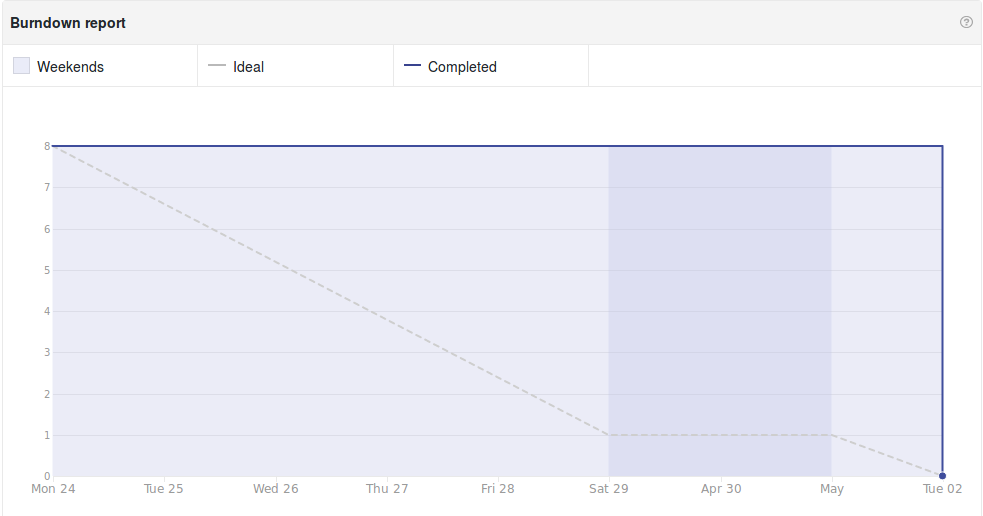
\includegraphics[width=\textwidth,height=7cm,keepaspectratio=true]{a_burndown_0}
    \caption[Gráfico burndown de la iteración 0]{Gráfico burndown de la iteración 0.}
    \label{fig:burndown0}
\end{figure}

En este caso el gráfico burndown de la figura \ref{fig:burndown0} muestra que todo el tiempo se fue con los problemas de la instalación de \textit{Unity} y que una vez completada el resto se terminó directamente.

\newpage
\subsection{Iteración 1: de 2-05-2017 hasta 7-05-2017}
En esta semana se empezó a trabajar con \textit{Unity}, se investigaron los ejemplos de prueba para crear el modelo del vehículo, se creó el primer algoritmo de planificación, el A*, y se investigó cómo se podían representar las rutas obtenidas en Unity llevándose a cabo su implementación.

Las tareas fueron:
\begin{itemize}
\item Crear el primer modelo de vehículo con movimiento y físicas de ruedas.
\item Crear el A*
\item Buscar cómo y realizar el dibujo de trayectorias.
\end{itemize}

\begin{figure}[htpb]
    \centering
    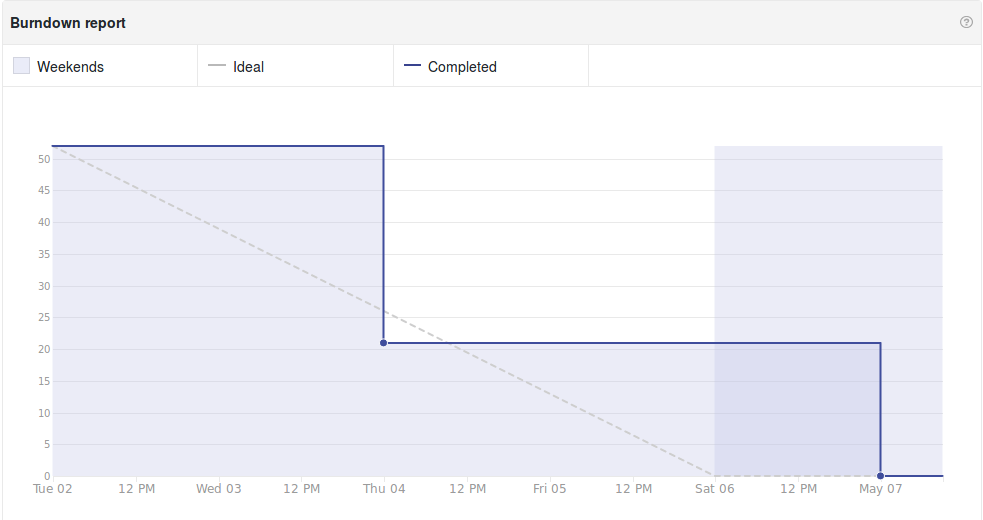
\includegraphics[width=\textwidth,height=7cm,keepaspectratio=true]{a_burndown_1}
    \caption[Gráfico burndown de la iteración 1]{Gráfico burndown de la iteración 1.}
    \label{fig:burndown1}
\end{figure}

El gráfico burndown de la figura \ref{fig:burndown1} muestra como se repartió el tiempo entre las dos tareas principales de estudiar los ejemplos de \textit{Unity} y realizar la implementación del A*.

\newpage
\subsection{Iteración 2: de 8-05-2017 hasta 15-05-2017}
Para esta semana se planificó terminar al A* y la representación de la trayectoria que se inició en la iteración anterior. Además, se investigó y se implementó la representación de los estados del A* para su visualización según se iba ejecutando el algoritmo. Por último, se planificó obtener el mapa de la escena de forma dinámica en tiempo de ejecución, que no fue posible debido a las limitaciones de la versión de \textit{Unity} utilizada, aunque se usó este trabajo y los conocimientos adquiridos sobre los \textit{Nav Mesh} para usarlos en el proyecto.

Las tareas fueron:
\begin{itemize}
\item Terminar A*.
\item Terminar la representación de la línea de trayectoria.
\item Crear la representación gráfica de la cuadrícula de los nodos de estado del A*.
\item Crear el mapa para el A* de forma dinámica según la escena.
\end{itemize}

\begin{figure}[htpb]
    \centering
    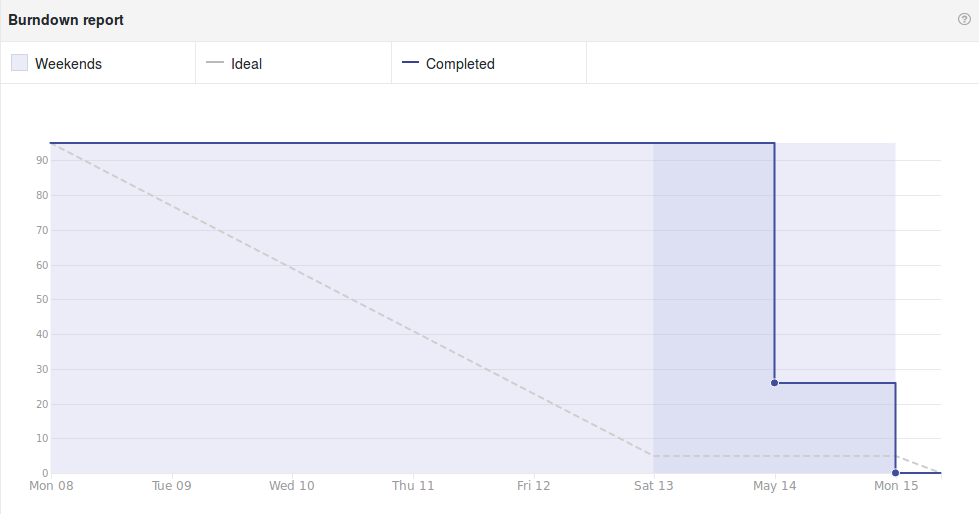
\includegraphics[width=\textwidth,height=7cm,keepaspectratio=true]{a_burndown_2}
    \caption[Gráfico burndown de la iteración 2]{Gráfico burndown de la iteración 2.}
    \label{fig:burndown2}
\end{figure}

El gráfico burndown de la figura \ref{fig:burndown2} muestra como la mayor parte del tiempo de esta iteración se utilizó en investigar el \textit{Nav Mesh} y la posible creación de los mapas de forma dinámica.

\newpage
\subsection{Iteración 3: de 16-05-2017 hasta 22-05-2017}
En esta iteración se implementó el \textit{Path Smoothing} para el suavizado de las rutas obtenidas. Se optimizó el rendimiento del A* a través del cambio de las estructuras de datos utilizadas, en concreto se buscó una implementación de una cola de prioridad. Se avanzó buscando documentación sobre \textit{PID Controller} para la próxima iteración, y se fue realizando la memoria con las secciones desarrolladas hasta ese momento.

Las tareas fueron:
\begin{itemize}
\item Implementar el \textit{Path Smoothing} al A*.
\item Optimizar el A*.
\item Buscar y leer documentación sobre el PID control.
\item Avanzar en la memoria.
\end{itemize}

\begin{figure}[htpb]
    \centering
    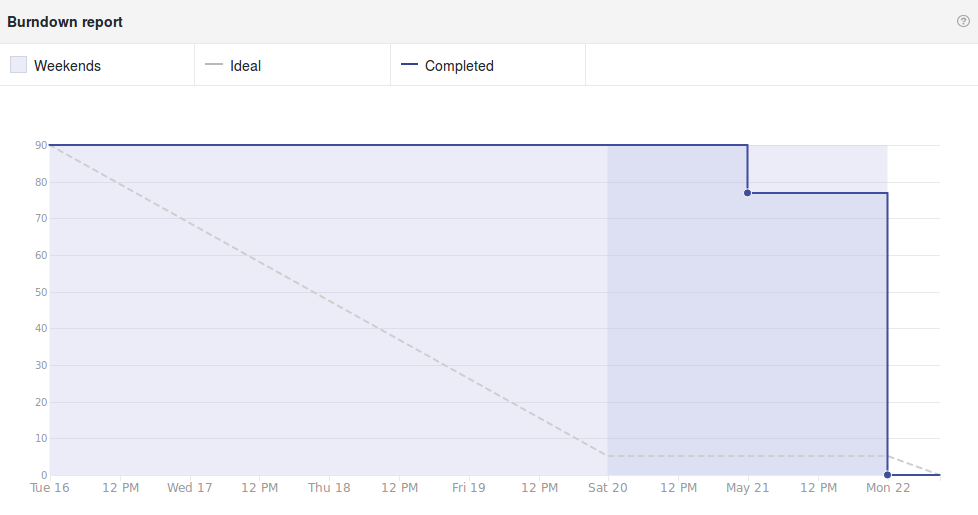
\includegraphics[width=\textwidth,height=7cm,keepaspectratio=true]{a_burndown_3}
    \caption[Gráfico burndown de la iteración 3]{Gráfico burndown de la iteración 3.}
    \label{fig:burndown3}
\end{figure}

En el gráfico burndown de la figura \ref{fig:burndown3} podemos observar que gran parte del tiempo de esta iteración se usó en la optimización del A* y en probar diferentes estructuras de datos, y la otra gran parte del tiempo se dedicó a realizar el \textit{Path Smoothing}.

\newpage
\subsection{Iteración 4: de 23-05-2017 hasta 30-05-2017}
Para esta iteración se utilizó la documentación de la semana anterior para desarrollar el \textit{PID Controller}. Para este semana se planificó realizar un \textit{PID Controller} para el control de las ruedas del vehículo.

También se implementaron dos nuevos algoritmos de búsqueda de rutas, el Theta* y el A* usando los vértices, que mejoraban al A* en la forma de las rutas obtenidas y en el rendimiento en el caso del A* de los vértices.

Se siguió realizando las secciones de la memoria correspondientes al trabajo realizado hasta el momento y se inició la creación de casos de test.

Las tareas fueron:
\begin{itemize}
\item Implementar \textit{PID Controller} para las ruedas y el motor.
\item Implementar algoritmo Theta*.
\item Implementar algoritmo A* con los vértices.
\item Avanzar con la memoria.
\item Empezar a crear casos de test.
\end{itemize}

\begin{figure}[htpb]
    \centering
    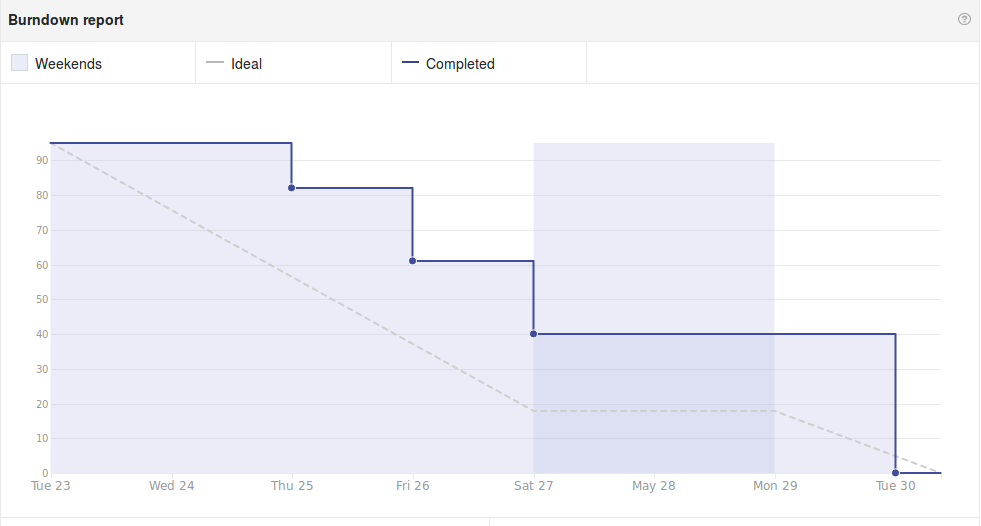
\includegraphics[width=\textwidth,height=7cm,keepaspectratio=true]{a_burndown_4}
    \caption[Gráfico burndown de la iteración 4]{Gráfico burndown de la iteración 4.}
    \label{fig:burndown4}
\end{figure}

En el gráfico burndown de la figura \ref{fig:burndown4} podemos ver como la semana se dividió principalmente entre la implementación de los algoritmos basados en al A* y la implementación del PID \textit{Controller}.

\newpage
\subsection{Iteración 5: de 31-05-2017 hasta 6-06-2017}
Para esta semana estaba planificado realizar un \textit{PID Controller} para el motor del vehículo, pero finalmente se decidió usar solamente el de las ruedas debido a que abarcaba los objetivos del proyecto por si mismo, moviendo el vehículo siguiendo la rutas obtenida, y utilizar en tiempo en otras tareas.

Se dedicó esta iteración a terminar las secciones de la memoria que se habían empezado las semanas anteriores, y a documentarse sobre el algoritmo \textit{Hybrid A*} para poder implementarlo en las siguientes iteraciones.

Las tareas fueron:
\begin{itemize}
\item Documentarse sobre la algoritmo Hybrid A* para implementarlo.
\item Avanzar en la memoria.
\end{itemize}

\begin{figure}[htpb]
    \centering
    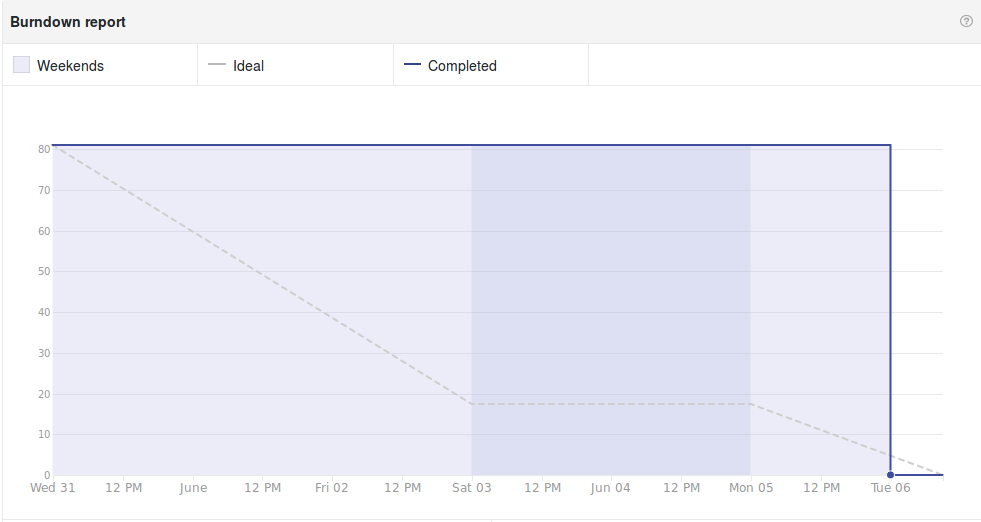
\includegraphics[width=\textwidth,height=7cm,keepaspectratio=true]{a_burndown_5}
    \caption[Gráfico burndown de la iteración 5]{Gráfico burndown de la iteración 5.}
    \label{fig:burndown5}
\end{figure}

En el gráfico burndown de la \ref{fig:burndown5} se muestra que el tiempo de esta semana se dedico a buscar documentación sobre el \textit{Hybrid A*}.

\newpage
\subsection{Iteración 6: de 7-06-2017 hasta 14-06-2017}
En esta iteración se implemento una primera versión del \textit{Hybrid A*}. Resulto complicado porque aún habiendo realizado buena parte de la documentación durante la semana anterior, no es un algoritmo que esté tan bien documentado y explicado como los anteriores. Finalmente se desarrollo una primera versión donde se calculaba la posición continua del vehículo y tenia en cuenta su rotación, pero resultaban rutas poco realistas y su movimiento a través del \textit{PID Controller} era limitado (por ejemplo, solo era capaz de ir adelante o hacia atrás no, cambiar de sentido).

También se utilizó parte del tiempo para realizar las correcciones a la memoria con los errores encontrados y las indicaciones de los tutores.

Las tareas fueron:
\begin{itemize}
\item Implementar el Algoritmo del \textit{Hybrid A*}.
\item Realizar las correcciones de la memoria.
\end{itemize}

\begin{figure}[htpb]
    \centering
    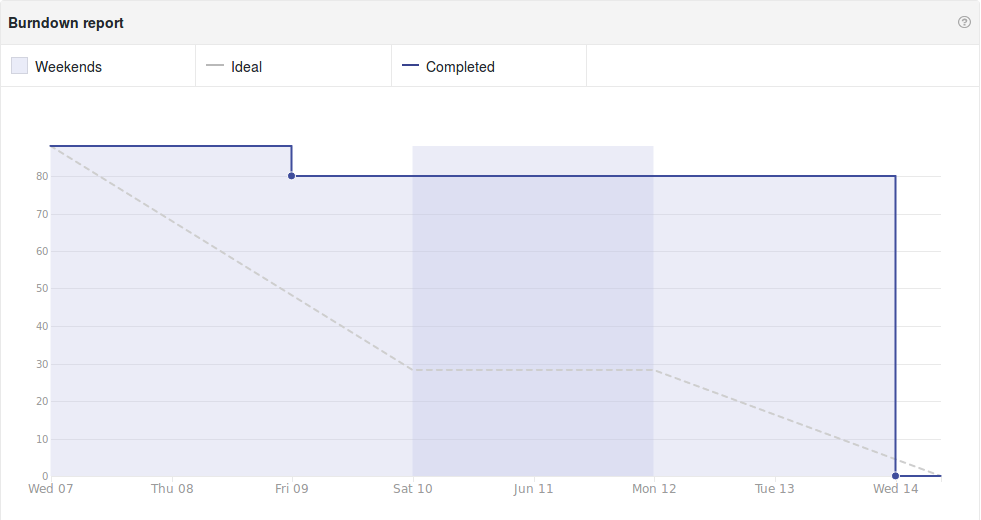
\includegraphics[width=\textwidth,height=7cm,keepaspectratio=true]{a_burndown_6}
    \caption[Gráfico burndown de la iteración 6]{Gráfico burndown de la iteración 6.}
    \label{fig:burndown6}
\end{figure}

En el gráfico burndown de la figura \ref{fig:burndown6} se muestra que tuvimos problemas en planificar las subtareas requeridas para le implementación del \textit{Hybrid A*} ya que aunque les estudiamos en la semana anterior fue complicado al ser un algoritmo del que no conocíamos nada de antemano y la dificultad de encontrar documentación detallada sobre le mismo.

\newpage
\subsection{Iteración 7: de 15-06-2017 hasta 19-06-2017}
Esta semana se dedicó a mejorar el \textit{Hybrid A*} para que el vehículo pudiera realizar maniobras. Para ello se modificaron las funciones del coste, se arreglaron los errores encontrados en la primera versión y se realizó un mapa de distancias. También fue necesario modificar el \textit{PID Controller} para que fuese capaz de seguir las rutas del \textit{Hybrid A*}. De esta manera se consiguió rutas más realistas que pudiera seguir el vehículo y que fuera capaz de realizar maniobras.

Además se siguió realizando la memoria con las secciones correspondientes al trabajo que se había ido realizando hasta el momento.

Las tareas fueron:
\begin{itemize}
\item Terminar el algoritmo del \textit{Hybrid A*}.
\item Avanzar en la memoria.
\end{itemize}

\begin{figure}[htpb]
    \centering
    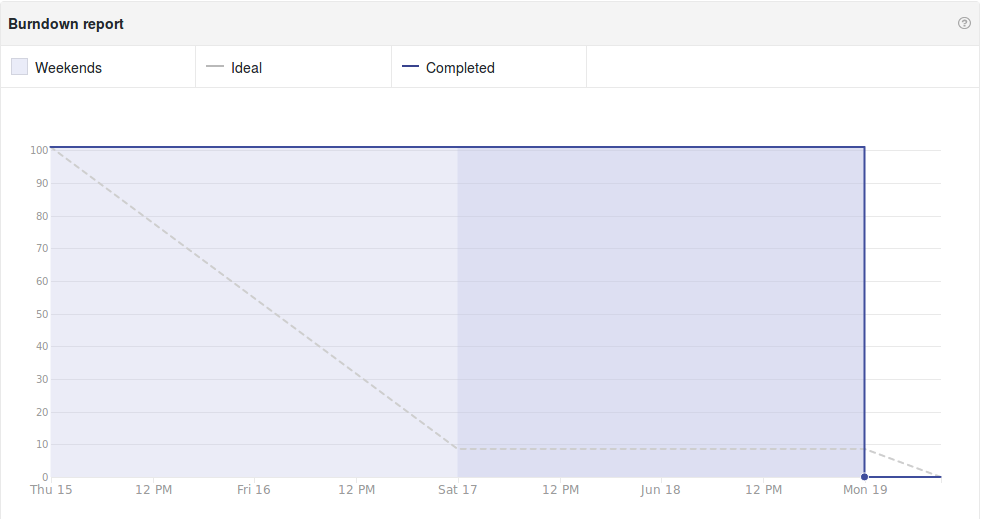
\includegraphics[width=\textwidth,height=7cm,keepaspectratio=true]{a_burndown_7}
    \caption[Gráfico burndown de la iteración 7]{Gráfico burndown de la iteración 7.}
    \label{fig:burndown7}
\end{figure}

Parecido a la semana anterior, el gráfico burndown de la figura \ref{fig:burndown7} muestra que una vez terminada la primera versión del \textit{Hybrid A*} que no funcionaba como deseábamos, se tuvo que investigar como poder arreglarlo sin tener las subtareas claras al inicio de la planificación.

\newpage
\subsection{Iteración 8: de 20-06-2017 hasta 26-06-2017}
Para esta semana principalmente se planificó terminar la memoria, añadiendo las últimas secciones, las imágenes, las tablas y los pseudocódigos.

Se finalizó el desarrollo del \textit{Hybrid A*} y se mejoró su rendimiento a través de la implementación de una nueva heurística que tiene en cuenta los obstáculos hasta la meta. Se mejoró el cálculo del coste corrigiendo los errores encontrados.

Las tareas fueron:
\begin{itemize}
\item Terminar la memoria y realizar las correcciones necesarias.
\item Mejorar heurística del \textit{Hybrid A*}.
\item Corregir errores en el cálculo de las heurísticas y el coste.
\end{itemize}

\begin{figure}[htpb]
    \centering
    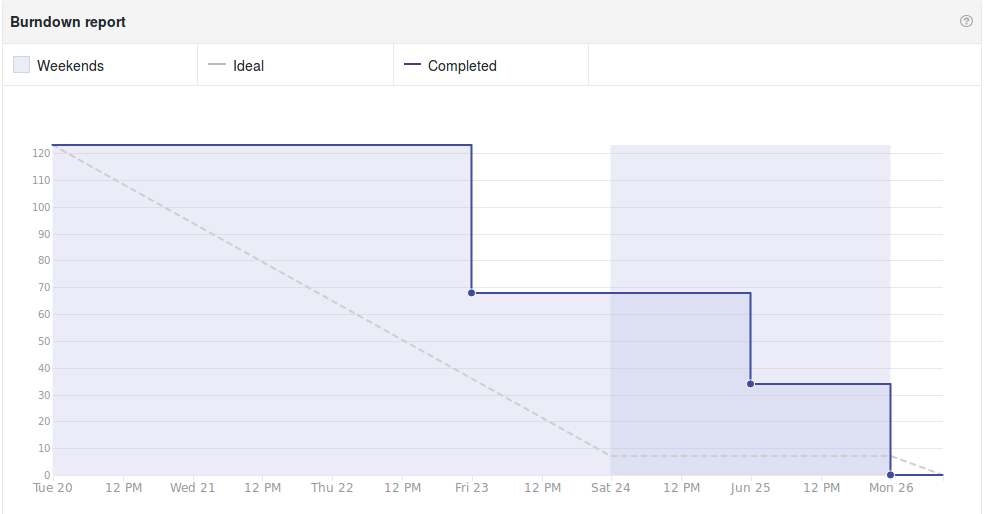
\includegraphics[width=\textwidth,height=7cm,keepaspectratio=true]{a_burndown_8}
    \caption[Gráfico burndown de la iteración 8]{Gráfico burndown de la iteración 8.}
    \label{fig:burndown8}
\end{figure}

El gráfico burndown de la figura \ref{fig:burndown8} muestra que en esta semana se planificó mejor las subtareas y el tiempo requerido por las mismas. La mayor parte del tiempo se dedicó a terminar la memoria y el resto a mejorar el \textit{Hybrid A*}.

\newpage
\subsection{Iteración 9: de 27-06-2017 hasta 3-07-2017}
En esta semana se termina el desarrollo del proyecto terminando las tareas pendientes.

Se realizaron los anexos y todas las secciones necesarias, se realizaron los vídeos con los resultados de distintas escenas, los casos de test, y la interfaz de usuario.

Las tareas fueron:
\begin{itemize}
\item Terminar los anexos.
\item Terminar los tests.
\item Implementar la GUI.
\item Realizar videos demostrativos.
\item Crear el póster de presentación.
\end{itemize}

\begin{figure}[htpb]
    \centering
    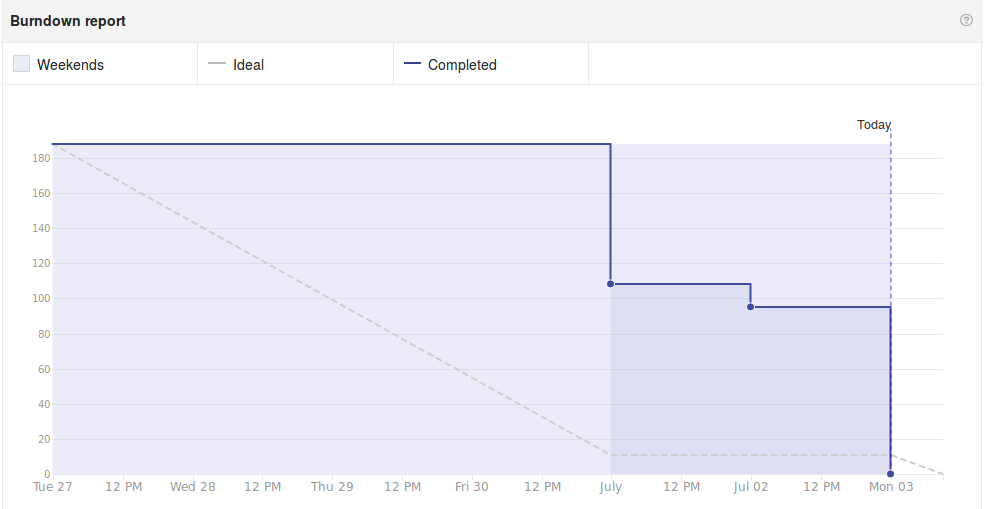
\includegraphics[width=\textwidth,height=7cm,keepaspectratio=true]{a_burndown_9}
    \caption[Gráfico burndown de la iteración 9]{Gráfico burndown de la iteración 9.}
    \label{fig:burndown9}
\end{figure}

En el gráfico burndown de la figura \ref{fig:burndown9} se puede observar que algunas tareas de la finalización del proyecto fueron más costosas de lo que se había planeado, ocupando más tiempo del planificado.

\newpage
\section{Estudio de viabilidad}

\subsection{Viabilidad económica}
En esta sección vamos a analizar el coste económico del proyecto y las posibles vías que pudiera tener para generar ingresos.

\subsubsection{Costes de personal}
El proyecto se ha llevado a cabo por una persona a tiempo completo durante dos meses. Hemos considerado que el salario neto rondaría los mil euros mensuales, y para calcular el coste total hemos considerado el porcentaje del salario de la Seguridad Social\footnote{Seguridad Social: \url{http://www.seg-social.es/Internet_1/Trabajadores/CotizacionRecaudaci10777/Basesytiposdecotiza36537/index.htm}} cuyo porcentaje es $31.2\%$ (contingencias comunes, contrato tiempo parcial y fondo de garantía social) , y del IRPF \footnote{IRPF: \url{http://www.agenciatributaria.es/static_files/AEAT/Contenidos_Comunes/La_Agencia_Tributaria/Informacion_institucional/Campanias/Retenciones_trabajo_personal/2017/Cuadro_tipo_retencion_2017.pdf}} cuyo porcentaje es $15\%$ para la elaboración de obras científicas.

\tablaSmall{Tabla de costes de personal}{l c}{tablacostepersonal}
{ \multicolumn{1}{l}{Coste} & Importe (\euro) \\}{ 
Salario mensual neto & 995.3 \\
IRPF & 277.5 \\
Seguridad Social & 577.2 \\
Salario Bruto & 1850 \\ \hline
\textbf{Total (2 meses)} & 3700 \\
}

En total el gasto por coste de personal para el proyecto es de 3700\euro.

\subsubsection{Costes de \textit{hardware}}
Para la realización del proyecto se ha utilizado un PC de sobremesa comprado en el año 2009 por un valor de 1000\euro \space aproximadamente. Vamos a considerar los meses transcurridos desde su compra como el tiempo para su amortización, en total 102 meses.

El coste amortizado de cada mes, por tanto, es de 9.8\euro, que por dos meses en total el coste del \textit{hardware} ha sido de 19.6\euro.

\subsubsection{Costes de \textit{software}}
Todo el \textit{software} utilizado ha sido \textit{software} libre o gratuito, incluido el sistema operativo que ha sido Xubuntu 16.04, por lo que el coste del \textit{software} ha sido de 0\euro.

\subsubsection{Otros costes}
La realización del proyecto lleva consigo otros costes adicionales que son necesarios para su realización. Hemos considerado el alquiler de un lugar para su realización de un coste aproximado de 500\euro\space mensuales, el coste del proveedor de internet necesario en 50\euro\space mensuales, y el coste de imprimir las memorias, el póster y los DVDs en 60\euro\space.

\tablaSmall{Tabla de otros costes}{l c}{tablaotroscostes}
{ \multicolumn{1}{l}{Otros costes} & Importe (\euro) \\}{ 
Internet & 50 \\
Impresos y DVDs & 60 \\
Alquiler & 500 \\ \hline
\textbf{Total (2 meses)} & 1160 \\
}

En total, el coste de estos otros gastos suman un total de 1160\euro\space.

\subsubsection{Total costes del proyecto}
El total de todos los costes del proyecto asciende a un total de 4879.6\euro.

\tablaSmall{Costes totales}{l c}{tablacostestotales}
{ \multicolumn{1}{l}{Costes} & Importe (\euro) \\}{ 
Personal & 3700 \\
\textit{Hardware} & 19.6 \\
\textit{Software} & 0 \\
Otros & 1160 \\ \hline
\textbf{Total} & 4879.6 \\
}

\subsubsection{Ingresos}
En un principio no se ha desarrollado la aplicación para que genere beneficios de ningún tipo, la intención del desarrollo ha sido de investigación y aprendizaje. De todas formas, la forma posible del obtener ingresos y rentabilizar el proyecto sería a través de la venta en la \textit{Unity Store}\footnote{Unity Store: \url{https://store.unity3d.com/}} de la implementación de los algoritmos como un \textit{asset} para otros proyectos.

Teniendo en cuenta el coste de 4879.6\euro, con un precio de 30\euro, y que \textit{Unity} en las condiciones legales\footnote{Unity Store, condiciones legales: \url{https://unity3d.com/es/legal/as_provider}} para usar su \textit{Store} retiene un $30\%$, no recuperaríamos la inversión hasta alcanzar las 233 unidades vendidas.

\subsection{Viabilidad legal}
En esta sección vamos a analizar la viabilidad legal de las licencias usadas en el proyecto así como las licencias con las que se distribuirá.

El motor \textit{Unity}\cite{unityweb} podemos usarlo libremente en su versión Personal siempre que no superemos unos ingresos de 100 mil dolares al año. En cuanto a \textit{Unity} y sus \textit{assets}, se pueden usar libremente dentro del proyecto\footnote{Unity Store EULA: \url{https://unity3d.com/es/legal/as_terms}} según los términos legales de la \textit{Unity Store}.

La librería externa que hemos usado ha sido la de la cola de prioridad en C\# \textit{High Speed Priority Queue for C Sharp}\footnote{Cola de prioridad: \url{https://github.com/BlueRaja/High-Speed-Priority-Queue-for-C-Sharp}}\cite{bluerajacola} que tiene una licencia de uso MIT \footnote{Licencia cola de prioridad: \url{https://github.com/BlueRaja/High-Speed-Priority-Queue-for-C-Sharp/blob/master/LICENSE.txt}} que nos permite usarla libremente incluso con fines comerciales.

Con lo cual, la limitaciones que nos encontramos en materia legal serían en caso de comercializar el proyecto, el límite de 100 mil dolares de \textit{Unity}, y tener en cuenta que los \textit{assets} solo se nos permite usarlos como una parte del proyecto, no podemos modificarlos y distribuirlos o venderlos de forma separada.

En cuanto a las licencia del código del proyecto se ha elegido la licencia GPL 3.0, de tal forma que los usos posteriores del código respeten la misma licencia y que deban distribuir el código fuente. Ya que no se ha desarrollado con una intención comercial, si no con intención de investigación y aprendizaje, y debido al uso que hemos dado al código abierto de otras fuentes (programas, ejemplos y la cola de prioridad) para desarrollarlo, consideramos que es la opción más adecuada.

En cuanto a la memoria y la documentación, hemos elegido por los mismo motivos una licencia \textit{Creative Commons} CC BY-NC\footnote{Licencias Creative Commons\url{https://creativecommons.org/licenses/?lang=es_ES}} que permite su uso en cualquier modo siempre que se reconozca la autoría y no se use en obras comerciales.